\documentclass{beamer} 
% \usetheme{Goettingen} 

\usepackage[latin1]{inputenc} 
\usepackage[ngerman]{babel} 
\usepackage[orientation=landscape,size=custom,width=16,height=9,scale=0.5]{beamerposter}
\usepackage{beamerthemeshadow}
\setbeamertemplate{enumerate items}[ball]

\begin{document}
\title{Producer/Consumer-Pattern}  
\author{Matthias Seifert}
\date{\today} 

\begin{frame}
\titlepage
\end{frame}
%tableofcontent
\section{die Aufgabe}
\begin{frame}
\begin{block}{die Aufgabe}
Mehrere Threads sollen miteinander kommunizieren k�nnen und f�r den
Austausch von Nachrichten einen Puffer verwenden.
\end{block}
\end{frame}
\begin{frame}
\centering
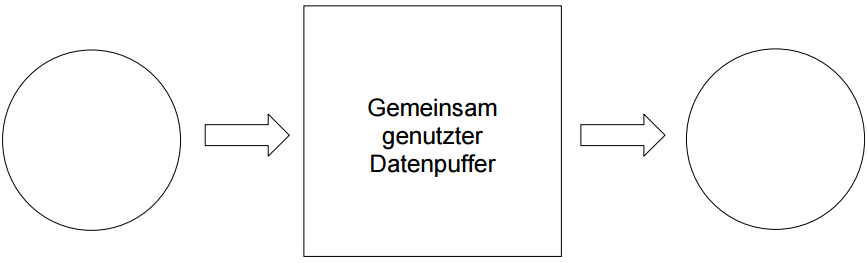
\includegraphics[width=.9 \textwidth]{img/1-1ohne.png}
\end{frame}

\begin{frame}
\centering
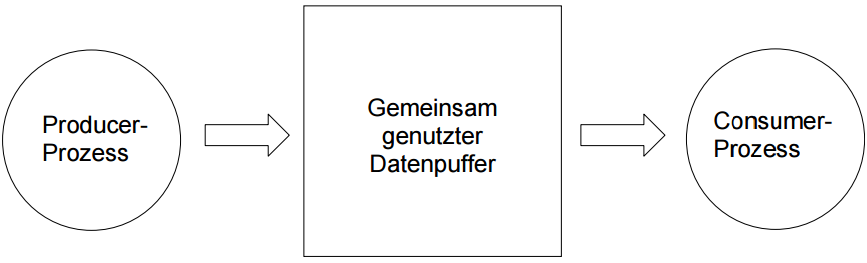
\includegraphics[width=.9 \textwidth]{img/1-1mit.png}
\end{frame}

\begin{frame}
\centering
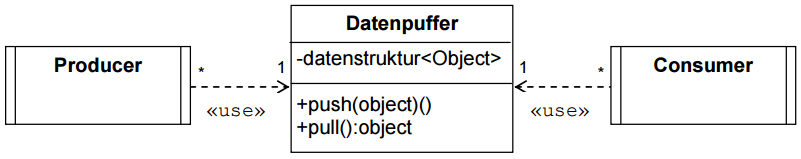
\includegraphics[width=.9 \textwidth]{img/klassendiagramm.png}
\end{frame}


\begin{frame}
\begin{block}{Problem}
Producer und Consumer d�rfen nicht gleichzeitig auf ein Element zugreifen
\end{block}
\end{frame}

\section{die L�sung}
\begin{frame}
\begin{block}{kritische Abschnitte sch�tzen}
\setbeamertemplate{itemize items}[square]
\begin{itemize}
  \item Semaphore
  \pause
  \item hier: Monitor
\pause
   \begin{itemize}
     \item<1-> zu sch�tzendes Element wird im Monitor verborgen
     \item<2-> Threads die einen blockierten Abschnitt betreten wollen werden
     blockiert.
 \end{itemize}
\end{itemize}
\end{block}
\end{frame}

\begin{frame}
\centering
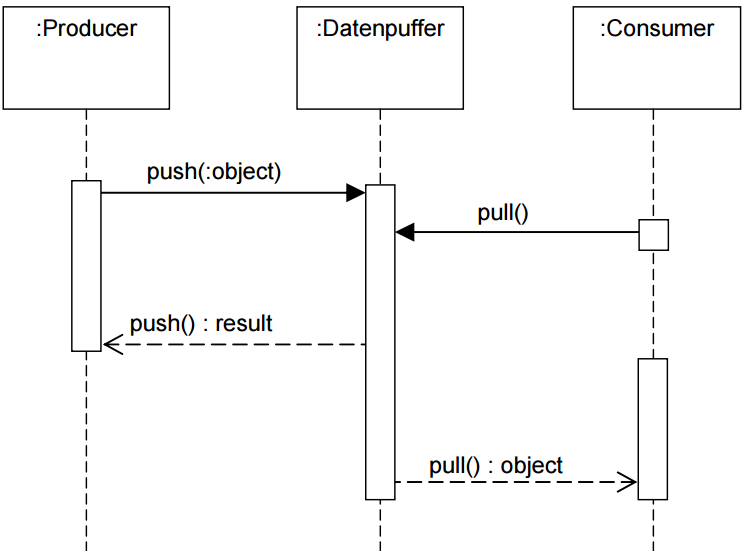
\includegraphics[height=.9 \textheight]{img/sequenz.png}
\end{frame}

\begin{frame}

\begin{columns}
\begin{column}{.5\textwidth}
\begin{block}{Vorteile}
\setbeamertemplate{itemize items}[square]
\begin{itemize}
  \item Producer und Consumer sind entkoppelt
  \item Anzahl Producer und Consumer kann unterschiedlich sein
  \item Konsistenz der Daten ist Gew�hrleistet
\end{itemize}
\end{block}
\end{column}
\begin{column}{.5\textwidth}
\begin{block}{Nachteile}
\setbeamertemplate{itemize items}[square]
\begin{itemize}
  \item Unbekannte Ausf�hrungsreihenfolge bei Freigabe von Element
\end{itemize}
\end{block}
\end{column}
\end{columns}
\end{frame}

\section{�hnliche Muster}
\subsection{Pipes \& Filters}
\begin{frame}

\begin{columns}
\begin{column}{.5\textwidth}
\begin{block}{Pipes \& Filters}
\setbeamertemplate{itemize items}[square]
\begin{itemize}
\item Sonderfall mit einem Producer und einem Consumer
\item Pipes = Pufferspeicher
\end{itemize}
\end{block}
\end{column}
\begin{column}{.5\textwidth}
\centering

\includegraphics[width=.3 \textwidth]{img/pipesandfilter.png}
\end{column}
\end{columns}
\end{frame}


\subsection{Guarded Suspension}
\begin{frame}

\begin{block}{Guarded Suspension}
\setbeamertemplate{itemize items}[square]
\begin{itemize}
\item Objekt muss zum Objektaufruf in definiertem Zustand sein
\item zugreifende Objekte m�ssen warten bis das Objekt in diesem Zustand ist
\end{itemize}
\end{block}

\end{frame}



% \subsection{Guarded Suspension}
% \begin{frame}
% asd
% \end{frame}




% 
% \frame{\frametitle{Firmenstrukturen}
% \begin{columns}
% \begin{column}{.5\textwidth}
% \begin{block}{levigo systems gmbh}
%   \begin{itemize}
%   \item Systemhaus
%   \item Aufbau und Betrieb von IT-Infrastruktur
%   \item 20 Mitarbeiter
%   \item Kunden aus dem Mittelstand
%   \end{itemize}
% \end{block}
% \end{column}
% \pause
% \begin{column}{.5\textwidth}
% \begin{block}{levigo solutions gmbh}
%  \begin{itemize}
%  \item Softwareentwicklung
%   \item Produkte: jadice-Produktfamilie
%   \item 18 Mitarbeiter
%   \item Kunden: Banken, Versicherungen
%   \end{itemize}
% \end{block}
% \end{column}
% \end{columns}
% }
% 
% \section{die Produkte}
% \frame{\frametitle{�bersicht}
% \begin{itemize}
%   \item Die jadice-Produktfamilie
%   \begin{itemize}
% \item Dokumentenmanagement
% \pause
% \item Plattformunabh�ngig (passende JVM vorausgesetzt)
% \pause
% \item Integrationsfreundlich
% \end{itemize}
% \end{itemize}
% }
% 
% \subsection{Server}
% \frame{\frametitle{jadice-Server}
%   \begin{columns}[T]
%     \begin{column}{.5\textwidth}
% \begin{itemize}
%   \item Zentrale Dokumentenkonvertierung und -verwaltung
%   \item Archivierung von E-Mails
%     \end{itemize}
%     \end{column}
%     \begin{column}{.5\textwidth}
% 
% \includegraphics[width=\textwidth]{server.jpg}
% 
%     \end{column}
%   \end{columns}
% }
% 
% \subsection{Viewer}
% \frame{\frametitle{jadice-Viewer}
% \begin{columns}[T]
% \begin{column}{.5\textwidth}
% \begin{itemize}
%   \item Unterst�tzt �ber 18 Dateiformate
%   \item kompatibel zu ImageIO-Plug-Ins
%   \item Effizient auch bei gro�en Dokumenten
%   \item Revisionssicheres Einf�gen von Annotationen
% \end{itemize}
% 
% \end{column}
% \begin{column}{.5\textwidth}
% \includegraphics[height=.8\textheight]{JadiceViewer.png}
% \end{column}
% \end{columns}
% }
% 
% \subsection{web toolkit}
% \frame{\frametitle{jadice web toolkit}
% 
% 
% \begin{columns}[T]
% \begin{column}{.5\textwidth}
% \begin{itemize}
%   \item Ben�tigt clientseitig keine JVM
%   \item L�uft komplett im Browser ohne weitere Plug-Ins
%   \item Anpassbares Styling
%   \item
%   {\href{http://webtoolkit.levigo.de:8080/enterprise/}{\underline{Webtoolkit
%   Demo}}}
% \end{itemize}
% 
% \end{column}
% \begin{column}{.5\textwidth}
% \includegraphics[width=\textwidth]{webtoolkit.png}
% \end{column}
% \end{columns}
% }
% \section{das Projekt}
% \subsection{das Problem}
% \begin{frame}
% \frametitle{das Problem}
% Kein direkter Zugriff auf die installierten Drucker aus dem
% Browser
% 
% \end{frame}
% 
% \begin{frame}
% \frametitle{Architektur}
% \begin{columns}
% \begin{column}{.5\textwidth}
% Umgehung der Sandbox mit einer eigenen Server/Client-Architektur
% \end{column}
% \pause
% \begin{column}{.5\textwidth}
% \includegraphics[height=.8\textheight]{architektur.png}
% \end{column}
% \end{columns}
% \end{frame}
% 
% \begin{frame}[fragile]
% \frametitle{Google Protobuffers}
% \begin{columns}
% \begin{column}{.5\textwidth}
% \begin{itemize}
%   \item Sprachunabh�ngig
%   \pause
%   \item einfach einzubinden
%   \pause
%   \item $\frac{1}{10}$ bis $\frac{1}{3}$ so gro� wie XML\footnotemark
%   \item 20-100 mal schneller\footnotemark[1]
%   \item Ver�ffentlicht unter BSD-Lizenz
% \end{itemize}
% \end{column}
% \pause
% \begin{column}{.5\textwidth}
% \begin{block}{sample.proto\footnotemark}
% \begin{verbatim}
% message SearchResponse {
%   repeated Result result = 1;
% }
% message Result {
%   required string url = 1;
%   optional string title = 2;
%   repeated string snippets = 3;
% }
% \end{verbatim}
% \end{block}
% \end{column}
% \end{columns}
% \footnotetext[1]{Quelle:
% \href{https://developers.google.com/protocol-buffers/docs/overview}{https://developers.google.com/protocol-buffers/docs/overview}}
% \footnotetext[2]{Quelle:
% \href{https://developers.google.com/protocol-buffers/docs/proto}{https://developers.google.com/protocol-buffers/docs/proto}}
% 
% 
% 
% \end{frame}
% \begin{frame}
% \frametitle{Netty}
% \begin{itemize}
%   \item Netzwerk-Framework
% \pause
%   \item Vorbereitete Protobuffer-Integration
% \pause
%   \item Einfach einzubinden
% \pause
%   \item Ver�ffentlicht unter Apache 2.0-Lizenz
% \end{itemize}
% \end{frame}
% % 
% % \begin{frame}
% % \frametitle{Ausblick}
% % \begin{itemize}
% %   \item {Integration des Printagent als Browser-Plugin}
% %   \pause
% %   \item {Getrennte Quellen f�r Dokumente und eingebettete Bilder oder
% %   Schriftarten}
% %   \pause
% % \end{itemize}
% % \end{frame}
% % 
% % \begin{frame}
% % 
% % \end{frame}
% % 
% % 
% % \begin{frame}
% % \frametitle{Digitale Inklusion - technische L�sungen zur Inklusion in der
% % digitalen Welt}
% % \begin{itemize}
% %   \item {Rechtliche Aspekte (UNO-Behindertenrechtskonvention /
% % Gesetzgebung in Deutschland / rechtlicher Rahmen in anderen L�ndern)} 
% % \item{Umsetzung der rechtlichten Vorgaben} 
% % \item{barrierefreie Dokumente PDF/UA (ISO 14289-1)}
% % \begin{itemize}
% % \item{Anforderungen an die Dokumente}
% % \item{Anforderungen an die erstellende Software}
% % \item{Anforderungen an die lesende Software}
% % \item{Umsetzung in Software} 
% % \item{Verbreitung}
% % 
% % \end{itemize}
% % 
% % \item{technische L�sungen (Screenreader, Braille-Zeilen)}
% % \item{barrierefreies Internet}
% % \end{itemize}
% % \end{frame}
% 
% 
% % \frame{\frametitle{blocs}
% % \begin{block}{title of the bloc}
% % bloc text
% % \end{block}
% % 
% % \begin{exampleblock}{title of the bloc}
% % bloc text
% % \end{exampleblock}
% % 
% % 
% % \begin{alertblock}{title of the bloc}
% % bloc text
% % \end{alertblock}
% % }
\end{document}